%%%%%%%%%%%%%%%%%%%%%%%%%%%%%%%%%%%%%%%%%%%%%%%%%%%%%%%%%%%%%%%%%%%%%%%%%%
%%%%%%%%%%%%%%%%%%%%%%%%%%%%%%%%%%%%%%%%%%%%%%%%%%%%%%%%%%%%%%%%%%%%%%%%%%
\chapter{Template}
\label{chap:zero}

\epigraph{\itshape  La volonté trouve, la liberté choisit. Trouver et choisir, c'est penser}{-- Victor Hugo}

\startcontents[chapters]

\printMyMinitoc

Texte après le mini-plan que vous pouvez mettre ici. Vous pouvez parler du contenu du chapitre et rappelez où nous en sommes dans l'avancement du mémoire.\newline
{\noindent \color{colorEPISEN-MEMOIRE}\textbf{Objectifs}}:
\begin{itemizeEPISEN}
	\item Réviser les bases ...
	\item Analyser ... 
	\item Rappeler ...
\end{itemizeEPISEN}

\fancyhead[LE]{\textsc{\chaptername~\thechapter}}

%%%%%%%%%%%%%%%%%%%%%%%%%%%%%%%%%%%%%%%%%%%%%%%%%%%%%%%%%%%%%%%%%%%%%%%%%%
%%%%%%%%%%%%%%%%%%%%%%%%%%%%%%%%%%%%%%%%%%%%%%%%%%%%%%%%%%%%%%%%%%%%%%%%%%

\section{Un peu de maths}

Rappel du glossaire si besoin~: \Gls{latex}. Suite test acronyme llm. prefixe. Inutile de mettre des liens vers le glossaire partout mais les première fois où un mot apparait (ou à des endroits où l'on craint que le relecteur puisse avoir oublier la signification) est très très utile et fortement recommandé.

%\lipsum[11] 

\begin{definition}[Un truc.]
On définit ici ce qu'est un truc avec $\sqrt{x}=\int_{i=0}^n \frac{1}{\log{x}}$
\end{definition}

\begin{definition}[Un bidule.]
On définit ici ce qu'est un bidule avec~:
\[
\sum_{i=0}^n x+i^{n \times n}
\]
\end{definition}

\begin{lemma}[Un premier résultat.]
\label{lemma:one}
Je crois que~:
\[
\left \{
   \begin{array}{r c l}
      AB  & = & 192 \\
      C   & = & 5\,896 \\
      DEF & = & 0,5
   \end{array}
   \right.
\]
\end{lemma}

\begin{lemma}[Un autre résultat.]
\label{lemma:second}
Et même que~:
\[
1+(-1)^n=\begin{cases}
			0, & \text{if $n$ odd}\\
            2, & \text{otherwise}
		 \end{cases}
\]
\end{lemma}




On peut en déduire la proposition suivante~:

 \begin{proposition}[Une proposition !]
 \label{prop:maPropo1}
 $\empty$\\
 \indent Franchement, c'est beau non ?
 \[
  A_{m\times n} \equiv
  \left[ {\begin{array}{cccc}
    a_{11} & a_{12} & \cdots & a_{1n}\\
    a_{21} & a_{22} & \cdots & a_{2n}\\
    \vdots & \vdots & \ddots & \vdots\\
    a_{m1} & a_{m2} & \cdots & a_{mn}\\
  \end{array} } \right]
\]
 \end{proposition}

Et enfin, pour terminer~:

 \begin{theorem}[Un résultat très important !]
 D'après Big Brother, $3=4$ et même $3 \neq 4$ !
 \end{theorem}

\begin{proof}
Donc, d'après le Lemme~\ref{lemma:one} et ~\ref{lemma:second}, on peut en déduire que~:
\begin{align*}
  f(\alpha) &= \beta^2\\
  g(\delta) &= \frac{1}{\varepsilon}\\
  F(x) &= \int^a_b \frac{1}{3}x^3
\end{align*}
puis avec la Proposition~\ref{prop:maPropo1}~:
\begin{equation}
  x = a_0 + \cfrac{1}{a_1 
          + \cfrac{1}{a_2 
          + \cfrac{1}{a_3 + \cfrac{1}{a_4} } } }
\end{equation}
Ce qui confirme que~:

\begin{tikzpicture}[shorten >=1pt,node distance=2cm,on grid,auto, every node/.style={scale=0.75}, scale=0.75] 
   \node[state,initial] (q_0)   {$q_0$}; 
   \node[state] (q_1) [above right=of q_0] {$q_1$}; 
   \node[state] (q_2) [below right=of q_0] {$q_2$}; 
   \node[state,accepting](q_3) [below right=of q_1] {$q_3$};
    \path[->] 
    (q_0) edge  node {1} (q_1)
          edge  node [swap] {1} (q_2)
    (q_1) edge  node  {1} (q_3)
          edge [loop above] node {0} ()
    (q_2) edge  node [swap] {0} (q_3) 
          edge [loop below] node {1} ();
\end{tikzpicture}
\end{proof}

%\lipsum[12] 

\noindent Pour illustrer ce théorème~:
\begin{example}
1=2
\end{example}

\section{Quelques items}

%\lipsum[13]

\noindent Une petite liste~:
\begin{itemize}
\item Des items
\item Standards
\end{itemize}

\noindent Une petite liste~:
\begin{enumerate}
\item Liste
\item Standard
\end{enumerate}

\noindent Une petite liste EPISEN~:
\begin{itemizeRondEPISEN}
\item Des items
\item EPISEN
\end{itemizeRondEPISEN}

\noindent Une autre petite liste EPISEN~:
\begin{enumerateEPISEN}
\item Des items
\item EPISEN
\end{enumerateEPISEN}

%\lipsum[7]

\subsection{Titre subsection 1}


Vous trouverez un exemple de tableau de données à mettre dans ce manuscrit
mais aussi dans le poster et dans le diaporama à la Figure~\ref{fig:tab1}.

On peut aussi mettre des images (ou des figures gnuplot, voir des tutos), pour faire des figures et compléter le poster/diaporama. Cela est visible, par exemple, à la Figure~\ref{fig:logo}. 

\phantomsection
\addcontentsline{toc}{section}{Mon boulot à moi}
\section*{Mon boulot à moi}

\begin{figure}[!t]
\begin{center}
\input{../ShareText/tab1.tex}
\end{center}
\caption{Un exemple de tableau dans tout les supports.}
\label{fig:tab1}
\end{figure}


\begin{figure}[!t]
\begin{center}
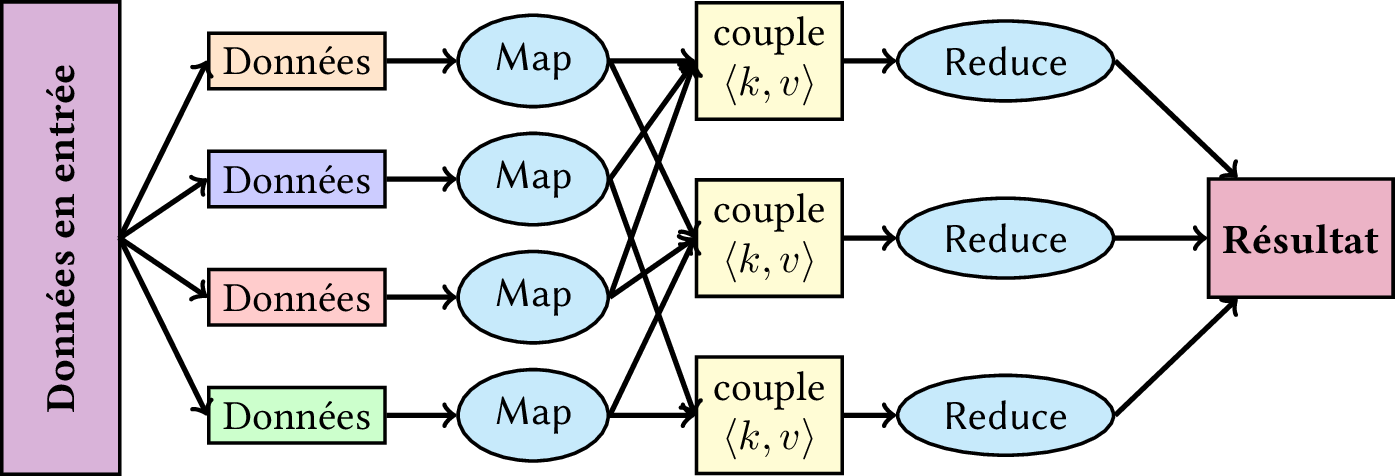
\includegraphics[height=5cm]{../images/Mapreduce.png}
\end{center}
\caption{Un exemple de figure avec dessin (png).}
\label{fig:logo}
\end{figure}

Cela est bien sûr aussi possible pour un listing de points importants que l'on souhaite voir dans ce manuscrit ainsi que dans le diaporama ou le poster. Exemple, ll est très important de~:
\input{../ShareText/listing1.tex}

On peut aussi mettre faire cela pour de jolies formules mathématiques dont on peut changer le contenu dans tout les supports si cela est dans un fichier séparé. Exemple~:
\input{../ShareText/maths1.tex}

Plutôt pratique non ?

\begin{itemize}
\item \underline{souligné}
\item {\bf en gras} ou \textbf{text}
\item {\it italique} ou \textit{text}
\end{itemize}

\phantomsection
\addcontentsline{toc}{section}{Plan}
\section*{Plan}
Et on n'oublie pas le plan du mémoire à la fin de l'introduction. Exemple~:
Nous parlerons de ... au Chapitre~\ref{chap:one} avec au début dans la Section~\ref{sec:one:one} à la page \pageref{sec:one:one} puis de ... dans la Section~\ref{sec:one:two} à la page \pageref{sec:one:two}. Dans le Chapitre~\ref{chap:two} nous continuerons à analyser... notamment avec l'exemple de blibli dans la Section~\ref{sec:two:one} à la page \pageref{sec:two:one} et puis le cas particulier de blabla dans la Section~\ref{sec:two:two} à la page \pageref{sec:two:two}.


\textit{etc.}

Et nous terminerons par la Conclusion à la page \pageref{chap:conclu}.

Il est à noter que vous trouverez certains codes dans l'Annexe~\ref{annexe:one} à la page \pageref{annexe:one} et tout les données dans l'Annexe~\ref{annexe:two} à la page \pageref{annexe:two}.


\subsubsection{Un exemple de sous-sous-section}

%\lipsum[15]

%\lipsum[18]

\subsubsection{Un autre exemple de sous-sous-section}

%\lipsum[19]

%\lipsum[20]


\subsection{Titre subsection 2}

%\lipsum[16]

%\lipsum[17]

\begin{figure}[!t]
\begin{center}
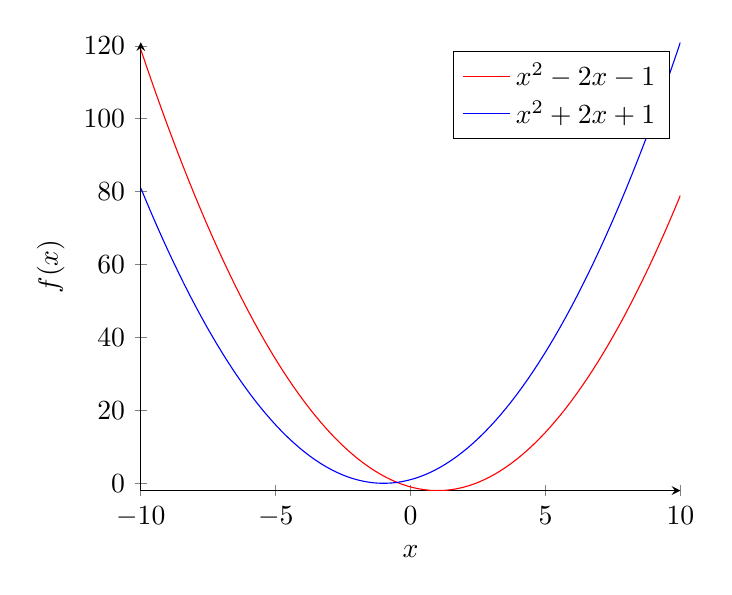
\begin{tikzpicture}
\begin{axis}[
    axis lines = left,
    xlabel = \(x\),
    ylabel = {\(f(x)\)},
]
%Below the red parabola is defined
\addplot [
    domain=-10:10, 
    samples=100, 
    color=red,
]
{x^2 - 2*x - 1};
\addlegendentry{\(x^2 - 2x - 1\)}
%Here the blue parabola is defined
\addplot [
    domain=-10:10, 
    samples=100, 
    color=blue,
    ]
    {x^2 + 2*x + 1};
\addlegendentry{\(x^2 + 2x + 1\)}

\end{axis}
\end{tikzpicture}
\end{center}
\caption{Un test avec pgfplot.}
\label{fig:test1}
\end{figure}


\begin{figure}[!t]
\begin{center}
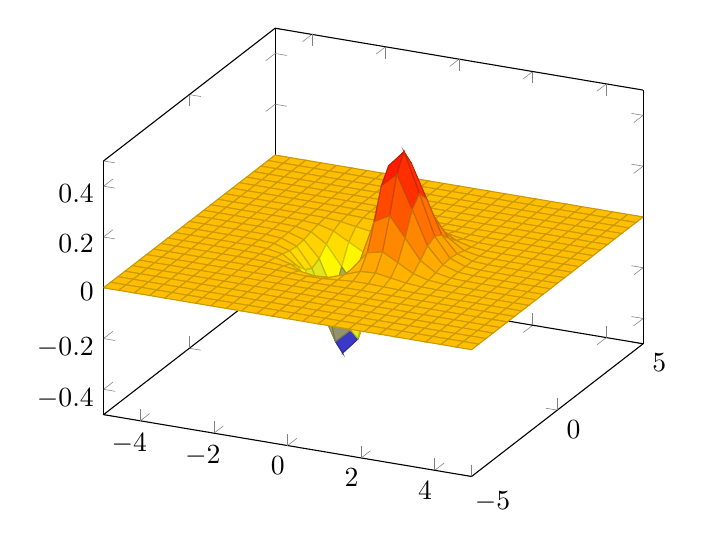
\begin{tikzpicture}
\begin{axis}
\addplot3[
    surf,
]
{exp(-x^2-y^2)*x};
\end{axis}
\end{tikzpicture}
\end{center}
\caption{Un autre test avec pgfplot.}
\label{fig:test2}
\end{figure}



\begin{figure}[!t]
\begin{center}
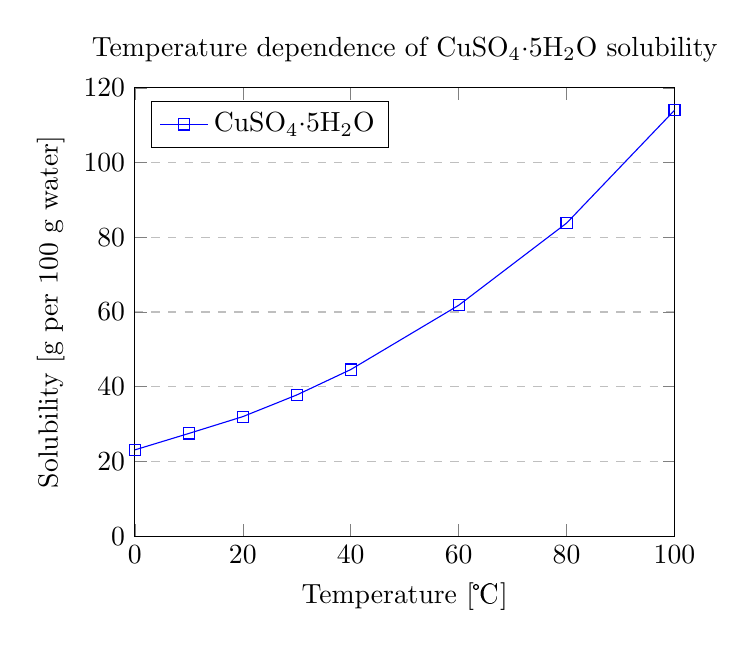
\begin{tikzpicture}
\begin{axis}[
    title={Temperature dependence of CuSO\(_4\cdot\)5H\(_2\)O solubility},
    xlabel={Temperature [\textcelsius]},
    ylabel={Solubility [g per 100 g water]},
    xmin=0, xmax=100,
    ymin=0, ymax=120,
    xtick={0,20,40,60,80,100},
    ytick={0,20,40,60,80,100,120},
    legend pos=north west,
    ymajorgrids=true,
    grid style=dashed,
]
\addplot[
    color=blue,
    mark=square,
    ]
    coordinates {
    (0,23.1)(10,27.5)(20,32)(30,37.8)(40,44.6)(60,61.8)(80,83.8)(100,114)
    };
    \legend{CuSO\(_4\cdot\)5H\(_2\)O}
\end{axis}
\end{tikzpicture}
\end{center}
\caption{Un graph de mesures avec pgfplot.}
\label{fig:test3}
\end{figure}


\begin{figure}[!t]
\begin{center}
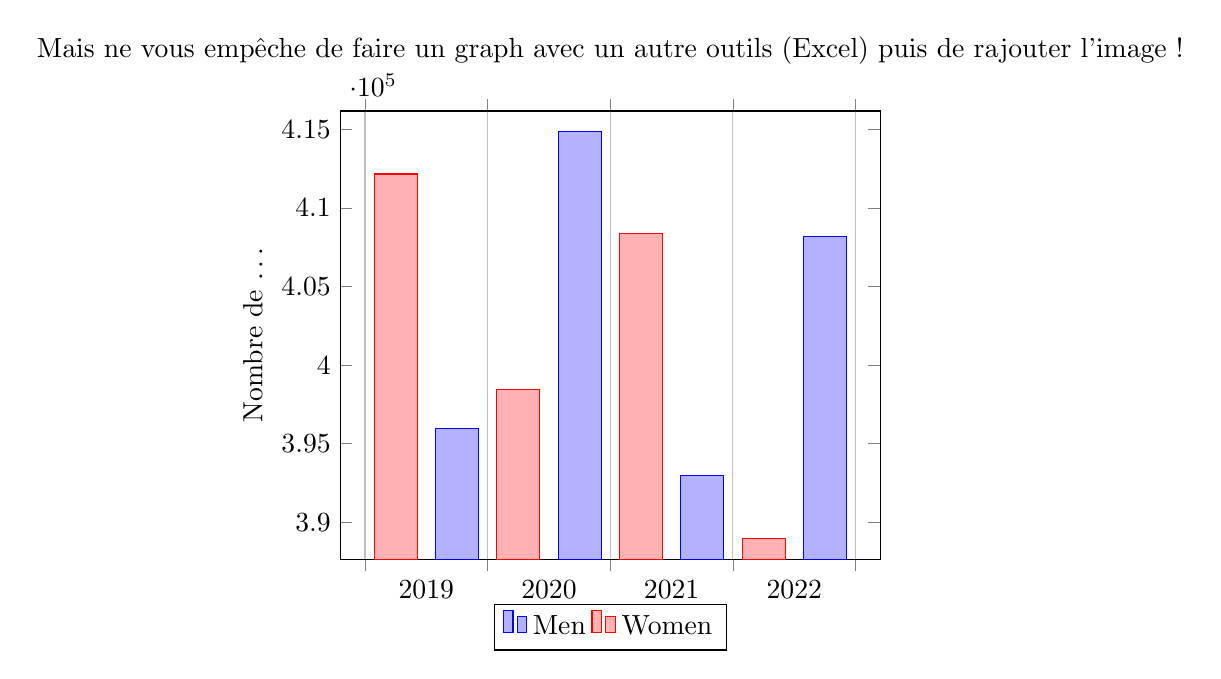
\begin{tikzpicture}
\begin{axis}[
title style={at={(0.5,1.15)},anchor=north},
title={Mais ne vous empêche de faire un graph avec un autre outils (Excel) puis de rajouter l'image !},
  x tick label style={
    /pgf/number format/1000 sep=},
  ylabel={Nombre de \( \ldots \) },
  xlabel=Années,
  enlargelimits=0.05,
  legend style={at={(0.5,-0.1)}, anchor=north, legend columns=-1},
  ybar interval=0.7,
]
%men
\addplot 
  coordinates { (2022,408184) (2021,393007) (2020,414870) (2019,395972) (2018,400000) }; %2018, bidon, juste affichage de 2019
%women
\addplot 
  coordinates { (2022,388950) (2021,408348) (2020,398449) (2019,412156) (2018,400000) }; %2018, bidon, juste affichage de 2019
\legend{Men,Women}
\end{axis}
\end{tikzpicture}
\end{center}
\caption{Un dernier graph avec pgfplot. }
\label{fig:test4}
\end{figure}


%%%%%%%%%%%%%%%%%%%%%%%%%%%%%%%%%%%%%%%%%%%%%%%%%%%%%%%%%%%%%%%%%%%%%%%%%%
%%%%%%%%%%%%%%%%%%%%%%%%%%%%%%%%%%%%%%%%%%%%%%%%%%%%%%%%%%%%%%%%%%%%%%%%%%

\epigraph{\itshape Si resté est ce texte, 0/20 tu auras bien mérité}{-- Gava Yoda}


Texte après le mini-plan que vous pouvez mettre ici. Vous pouvez parler du contenu du chapitre et rappelez où nous en sommes dans l'avancement du mémoire.\newline
{\noindent \color{colorEPISEN-MEMOIRE}\textbf{Objectifs}}:
\begin{itemizeEPISEN}
	\item Réviser les bases ...
	\item Analyser ... 
	\item Rappeler ...
\end{itemizeEPISEN}

\fancyhead[LE]{\textsc{\chaptername~\thechapter}}

%%%%%%%%%%%%%%%%%%%%%%%%%%%%%%%%%%%%%%%%%%%%%%%%%%%%%%%%%%%%%%%%%%%%%%%%%%
%%%%%%%%%%%%%%%%%%%%%%%%%%%%%%%%%%%%%%%%%%%%%%%%%%%%%%%%%%%%%%%%%%%%%%%%%%


\section{Titre section 1 (second chapitre)}

%lipsum[4] 

%lipsum[5] 

\section{Des codes}

%lipsum[6]

\subsection{Java}

%lipsum[7]

\begin{java}
public class {
	...
	public static void main(String arg){
		System.out.println("sdmklfjsdfj dfsdf ");
		/* A loop */
		for(int i=0;i<n;i++)
			if (1=1)
				Toto.add(i)
	}
}
\end{java}

%lipsum[8]

\subsection{Code Python}

%lipsum[9]

On peut aussi mettre une barre devant les codes (exemple ci-dessous) et même
mettre dans des figures (voir Figure~\ref{fig:code1}). Cela fait beaucoup de couleur je trouve mais si vous aimez, ca fonctionne.

\begin{code}
\begin{python}
# Les listes :
maListeDeMeubles = ['table','chaise','frigo']
maListeDeMeubles.sort()  #Tri de la liste

# A loop et avec des maths $x=\int_{i=1}^n \sin{x}$
for unMeuble in maListeDeMeubles:
   print('longueur de la chaîne ', unMeuble, '=', len(unMeuble))

#les listes imbriquées:
laListeDesNombresPairs = [unNombre for unNombre in range(1000) if unNombre % 2 == 0]
print (laListeDesNombresPairs)

#Les dictionnaires :
unAnnuaire = {'Laurent': 6389565, 'Paul': 6356785}
for unNom, x in unAnnuaire.items():
   print("le nom %s a pour numéro de téléphone %d" %(unNom, x))


#Les tuples (n-uplet) : séquence constante
Couleur = ('Rouge', 'Bleu', 'Vert')
print(Couleur[0], Couleur[1],  Couleur[2])

PointDeReference = (100, 200)
print(" x0 = %d   y0 = %d "  %(PointDeReference[0],PointDeReference[1]))
\end{python}
\end{code}

%lipsum[10]

\subsection{Code R (maths)}

%lipsum[11]

\begin{R}
data <- read.table("data.dat", header = FALSE, sep = "")
M <- data.frame(n1, n2, m)
x <- 1:30

fib <- function(n) {
|	if (n < 2)
|	| n
|	else
|	| fib(n - 1) + fib(n - 2)
}

fib(10) # => 55

myfun <- function(S, F) {
|	data <- read.table(F)
|	plot(data$V1, data$V2, type="l")
|	title(S)
}

for(i in 1:length(species)) {
|	data <- read.table(file[i]) # lit les données
|	plot(data$V1, data$V2, type="l")
|	title(species[i]) # ajoute le titre
}

#Calculate CE for each counterparty
Value.A <- data.frame() #MTM value of each contract within cp A
# ...
for(i in 1:length(foo)){
|	if(isTrue(as.character(portfolio_data[i,1])=="A")==TRUE){
|	# ...
}
\end{R}

%lipsum[12]

\subsection{Code source sans formatage}

%lipsum[13]

Exemple d'un Makefile (mais mettez ce que vous voulez, du HTML, des scripts, la sortie
standard de votre shell, {\it etc.} ou du textt+maths)
\begin{codeExample}
\begin{small}
\begin{verbatim}
fast:
	pdflatex memoire.tex

memoire: all

manuscrit: memoire

all:
	pdflatex memoire.tex
	pdflatex memoire.tex

clean:
	rm -f memoire.pdf memoire.aux  memoire-blx.bib memoire.lot memoire.mtc0 	

allClean: clean
	rm -f *.pdf
\end{verbatim}
\end{small}
\end{codeExample}

%lipsum[14]

%lipsum[15]

\begin{figure}[!t]
\begin{code}
\begin{java}
public class {
|	...
|	public static void main(String arg){
|	|	System.out.println("sdmklfjsdfj dfsdf ");
|	|	/* A loop et avec des maths $x=\int_{i=1}^n \sin{x}$ */
|	|	for(int i=0;i<n;i++)
|	|	|	if (1=1)
|	|	|	|	Toto.add(i)
|	}
}
\end{java}
\end{code}
\caption{Un exemple de code Java dans une figure.}
\label{fig:code1}
\end{figure}

Et un exemple d'Algorithme~\ref{algo:level}. Vous pouvez faire une table des algorithme mais je laisse cela en exercice à ceux qui en auraient besoin...

\begin{algorithm}[!t]
\SetAlgoLined
\SetKwInOut{Input}{\color{colorEPISEN-MEMOIRE}input}
\SetKwInOut{Output}{\color{colorEPISEN-MEMOIRE}output}
\SetKwData{indegreeMap}{indegreeMap}
%\SetKwFunction{FindCompress}{FindCompress}
\Input{A boolean circuit $G$}
\Output{The level of each gate $v \in G$}
\BlankLine
inLevelMap $\leftarrow \{ (v\!\Rightarrow\!0) \ \ \forall v\!\in V_{in} \}$ \;
slice $\leftarrow [ v                 \ \ \forall v\!\in V_{in} ]$ \;
accu $\leftarrow \emptyset$ \;
numOfSlices $\leftarrow 0$ \;
\While{slice $\neq \emptyset$}{
	accu $\leftarrow$ accu $\oplus$ slice \;
	newSlice $\leftarrow$ $[]$ \;
	\For{v $\in$ slice}{
		\For{(v',e) $\in \mathbf{edges}(G,v)$}{
			inLevelMap[e] $\leftarrow$ inLevelMap[e]-1 \;
			\If{inLevelMap[e] $\neq 0$}{
				newSlice $\leftarrow$ newSlice $\oplus$ e
			}
		}
	}
	slice $\leftarrow$ newSlice \;
	numOfSlices++
}
\Return accu, numOfSlices-1

%$\{v: d \ for v, d in G.in_degree().items() if d > 0 \}$ \;
%\While{not at end of this document}{
%read current\;
%\eIf{understand}{
%go to next section\;
%current section becomes this one\;
%}{
%go back to the beginning of current section\;
%}
%}
\caption{Building the level of each gate.}
\label{algo:level}
\end{algorithm}

%lipsum[16]